
\section{Atividade 4}

Esta atividade consiste na modelagem e análise de um sistema de controle massa-mola-amortecedor. O sistema é controlado por um controlador proporcional e monitorado por um sensor de primeira ordem. O objetivo é analisar a estabilidade do sistema e determinar o limite crítico do sistema.


% ===============================================================
% Letra A =======================================================
\subsection{Parte (a): Descrição do Diagrama de Blocos}

\begin{figure}[H]
    \centering
    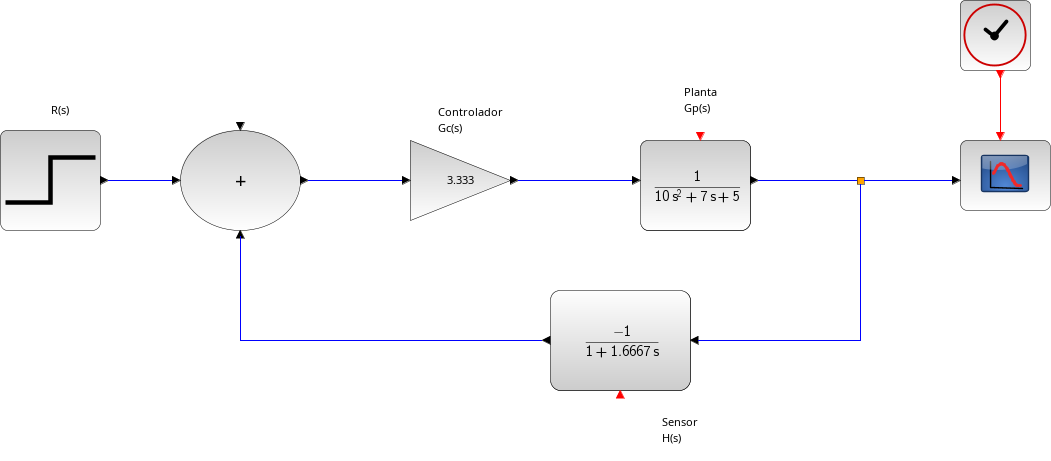
\includegraphics[width=0.8\textwidth]{atividades/4-atividade/assets/diagrama-blocos.png}
    \caption{Diagrama de blocos do sistema de controle proporcional.}
    \label{fig:diagrama_blocos}
\end{figure}

O diagrama de blocos apresentado na Figura~\ref{fig:diagrama_blocos} ilustra a configuração do sistema de controle:

\begin{itemize}
    \item \textbf{Controlador Proporcional (\(G_c(s)\))}: Com ganho de \(\frac{10}{3}\) = (\(3.333\)), o controlador ajusta a saída com base na diferença entre a referência e o sinal medido pelo sensor.
    \item \textbf{Planta (\(G_p(s)\))}: Representada pela função de transferência \(\frac{1}{10s^2 + 7s + 5}\), que descreve a dinâmica do sistema massa-mola-amortecedor.
    \item \textbf{Sensor (\(H(s)\))}: O sensor é modelado como um sistema de primeira ordem com a função de transferência \(\frac{1}{1 + 1.6667s}\), capturando a resposta da variável controlada com uma certa constante de tempo.
    \item \textbf{Soma (\(\Sigma\))}: Um somador que computa a diferença entre a referência e a saída do sensor, alimentando essa diferença para o controlador.
    \item \textbf{Feedback}: O loop de feedback é crucial para garantir que a saída do sistema esteja em conformidade com a entrada desejada.
\end{itemize}

O sistema é projetado para monitorar e ajustar a saída de modo a atingir um estado desejado, com foco na estabilidade e eficiência do controle.



% ===============================================================
% Letra B =======================================================
\subsection{Parte (b): Função de Transferência em Malha Fechada}

Para o sistema de controle proposto, primeiramente definimos os parâmetros físicos e as configurações do sistema. A planta é um sistema massa-mola-amortecedor, e o controlador utilizado é um controlador proporcional. O sensor é modelado por um sistema de primeira ordem. Os parâmetros são definidos como segue:

\begin{itemize}
    \item Massa, \(m = 10\, \text{kg}\)
    \item Coeficiente de amortecimento, \(c = 7\, \text{Ns/m}\)
    \item Constante da mola, \(k = 5\, \text{N/m}\)
\end{itemize}

O ganho do controlador proporcional, \(K\), é definido como:
\[ K = \frac{m}{3} \]

A constante de tempo do sensor, \(T_s\), é determinada por:
\[ T_s = \frac{m}{6} \]

As funções de transferência para a planta (\(G_p(s)\)), o sensor (\(H_s(s)\)), e o controlador proporcional (\(G_c(s)\)) são definidas da seguinte forma:
\begin{align*}
    G_p(s) & = \frac{1}{m s^2 + c s + k} = \frac{1}{10 s^2 + 7 s + 5} \\
    H_s(s) & = \frac{1}{T_s s + 1} = \frac{1}{\frac{10}{6} s + 1}     \\
    G_c(s) & = K = \frac{10}{3}
\end{align*}

\subsubsection{Código Scilab utilizado calcular a Função de Transferência em Malha Fechada}
\begin{lstlisting}[language=Scilab, caption=Código Scilab para calcular a função de transferência em malha fechada]
    // Definicao dos parametros
    s = poly(0, 's');
    m = 10;  // massa
    c = 7;   // coeficiente de amortecimento
    k = 5;   // constante da mola
    
    // Definicao das funcoes de transferencia
    K = m / 3;  // Ganho do controlador proporcional
    Ts = m / 6;  // Constante de tempo do sensor
    
    // Funcoes de Transferencia
    Gp = syslin('c', 1, m*s^2 + c*s + k);  // Planta
    Hs = syslin('c', 1, Ts*s + 1);  // Sensor
    Gc = syslin('c', K, 1);  // Controlador Proporcional
    
    // Funcao de Transferencia em Malha Fechada C(s)/R(s)
    sys = Gc * Gp / (1 + Gc * Gp * Hs);
    
    // Exibicao da Funcao de Transferencia em Malha Fechada
    disp("Funcao de Transferencia em Malha Fechada C(s)/R(s):");
    disp(sys);
    \end{lstlisting}



A função de transferência em malha fechada \(C(s)/R(s)\) é calculada pela integração dessas funções de transferência, resultando na seguinte expressão:
\[
    C(s)/R(s) = \frac{G_c(s) G_p(s)}{1 + G_c(s) G_p(s) H_s(s)}
\]

Após a simplificação e cálculos realizados pelo software Scilab, a função de transferência em malha fechada resultante é:
\[
    \frac{0.2 + 0.3333333s}{0.5 + 0.92s + 1.3s^2 + s^3}
\]

Esta função de transferência em malha fechada indica como o sistema responde à entrada \(R(s)\) dada a configuração de controle atual. A expressão mostra a relação entrada-saída considerando a realimentação do sensor e a ação do controlador proporcional.


% ===============================================================
% Letra C =======================================================

\subsection{Parte (c): Análise de Estabilidade com o Critério de Routh-Hurwitz}

Após calcular a função de transferência em malha fechada \(C(s)/R(s)\), o próximo passo é analisar a estabilidade do sistema de controle. Utilizamos o critério de Routh-Hurwitz para essa finalidade, que é uma técnica fundamental na teoria de controle para determinar a estabilidade de um sistema linear.


\subsubsection{Código Scilab para a Análise de Routh-Hurwitz}
\begin{lstlisting}[language=Scilab, caption=Código Scilab para calcular a matriz de Routh-Hurwitz]
    // Definicao dos parametros
    s = poly(0, 's');
    m = 10;  // massa
    c = 7;   // coeficiente de amortecimento
    k = 5;   // constante da mola

    // Definicao das funcoes de transferencia
    K = m / 3;  // Ganho do controlador proporcional
    Ts = m / 6;  // Constante de tempo do sensor

    // Funcoes de Transferencia
    Gp = syslin('c', 1, m*s^2 + c*s + k);  // Planta
    Hs = syslin('c', 1, Ts*s + 1);  // Sensor
    Gc = syslin('c', K, 1);  // Controlador Proporcional

    // Funcao de Transferencia em Malha Fechada C(s)/R(s)
    sys = Gc * Gp / (1 + Gc * Gp * Hs);

    // Extraindo o denominador da Funcao de Transferencia para Analise de Estabilidade
    den = sys.den;

    rh_matrix = routh_t(den);

    // Exibir a Matriz de Routh-Hurwitz
    disp("Matriz de Routh-Hurwitz:");
    disp(rh_matrix);
\end{lstlisting}


\subsubsection{Extração do Denominador da Função de Transferência}

A estabilidade de um sistema de controle pode ser analisada pelo estudo das raízes do polinômio característico do denominador da função de transferência em malha fechada. Estas raízes, também conhecidas como pólos do sistema, determinam como o sistema responde a diferentes entradas ao longo do tempo. A localização desses pólos no plano complexo indica se as respostas do sistema serão estáveis, instáveis ou em um estado de margem de estabilidade.

No caso do sistema considerado, a função de transferência em malha fechada resultante é calculada pelo produto e pela soma das funções de transferência do controlador proporcional, da planta e do sensor, estruturados como segue:
\[
    C(s)/R(s) = \frac{Gc \times Gp}{1 + Gc \times Gp \times Hs}
\]
A partir desta expressão, o denominador, que contém o polinômio característico do sistema, é dado por:
\[
    1 + Gc \times Gp \times Hs
\]
Expandindo e simplificando este produto usando os parâmetros e as funções definidas no código Scilab, o denominador da função de transferência em malha fechada é obtido. Este processo resulta em um polinômio em \(s\) que representa a combinação das dinâmicas do controlador, da planta e do sensor.

Para este sistema específico, utilizando os parâmetros dados, o denominador extraído e simplificado é:
\[
    0.5 + 0.92s + 1.3s^2 + s^3
\]
Este polinômio é então usado para a construção da matriz de Routh-Hurwitz, que é uma técnica clássica de análise de estabilidade, ajudando a determinar a presença de raízes com partes reais não negativas e, consequentemente, se o sistema é estável ou não.



\subsubsection{Cálculo da Matriz de Routh-Hurwitz}

Para construir a matriz de Routh-Hurwitz, utilizamos a função \texttt{routh\_t} que calcula essa matriz a partir do polinômio característico. A matriz de Routh-Hurwitz para o denominador do sistema é calculada e apresentada como segue:
\[
    \begin{array}{c|cc}
        s^3 & 1         & 0.92 \\
        s^2 & 1.3       & 0.5  \\
        s^1 & 0.5353846 & 0    \\
        s^0 & 0.5       &      \\
    \end{array}
\]

\subsubsection{Interpretação da Matriz de Routh-Hurwitz}

Os elementos da primeira coluna da matriz de Routh-Hurwitz indicam a estabilidade do sistema. Todos os elementos devem ser positivos para garantir estabilidade. A matriz mostra que todos os termos são positivos, sugerindo que o sistema é estável. Esta análise detalhada fornece confiança adicional na robustez do sistema sob a configuração de controle atual.

\subsubsection{Conclusão da Análise de Estabilidade}

A análise com a matriz de Routh-Hurwitz confirma que o sistema é estável sob as condições atuais. A positividade de todos os termos na primeira coluna da matriz assegura que não há raízes com partes reais positivas, o que implica em uma resposta do sistema estável e controlada. Essa conclusão é vital para garantir que o sistema opere de forma segura e eficaz, mantendo o desempenho desejado.

% ===============================================================
% Letra D =======================================================
\subsection{Parte (d): Análise de Estabilidade para Diferentes Valores de \(K\)}

A estabilidade do sistema de controle é investigada para uma variação do ganho \(K\) do controlador proporcional, substituído pelo parâmetro variável \(K\). Utilizamos a função de transferência em malha fechada definida pelos parâmetros físicos do sistema para determinar para quais valores de \(K\) o sistema é estável.

\subsubsection{Definição da Função de Transferência}
Com base nos parâmetros do sistema, a função de transferência da planta \(G_p(s)\) e do sensor \(H_s(s)\) são definidas como segue:

\[
    G_p(s) = \frac{1}{10 s^2 + 7 s + 5}
\]

\[
    H_s(s) = \frac{1}{\frac{10}{6} s + 1}
\]

\subsubsection{Função de Transferência em Malha Fechada}
A função de transferência em malha fechada \(T(s)\), considerando o controlador proporcional \(G_c(s) = K\), é dada por:

\[
    T(s) = \frac{K \cdot G_p(s)}{1 + K \cdot G_p(s) \cdot H_s(s)}
\]

Substituindo \(G_c(s)\), \(G_p(s)\), e \(H_s(s)\) com os valores acima, obtemos:

\[
    T(s) = \frac{K \left(\frac{1}{10 s^2 + 7 s + 5}\right)}{1 + K \left(\frac{1}{10 s^2 + 7 s + 5}\right) \left(\frac{1}{\frac{10}{6}s + 1}\right)}
\]

Multiplicando numerador e denominador pelo MMC dos denominadores das funções de transferência, obtemos:

\[
    T(s) = \frac{5Ks + 3K}{3K + 50s^3 + 65s^2 + 46s + 15}
\]
Esta função representa a resposta do sistema em função do ganho proporcional \(K\), onde \(K\) modula a entrada em função das dinâmicas combinadas da planta e do sensor.

\subsubsection{Construção da Matriz de Routh-Hurwitz}

A análise da estabilidade do sistema é feita através da matriz de Routh-Hurwitz, que é construída a partir do polinômio característico:
\[
    50s^3 + 65s^2 + 46s + 15 + 3K
\]

A estabilidade do sistema é analisada através da construção da matriz de Routh-Hurwitz para o polinômio característico derivado do denominador da função de transferência em malha fechada:
\[
    \begin{array}{c|cc}
        s^3 & 50                     & 46      \\
        s^2 & 65                     & 15 + 3K \\
        s^1 & \frac{150K - 2240}{65} & 0       \\
        s^0 & 15 + 3K                &         \\
    \end{array}
\]
Onde:
\[
    s^1 = \frac{150K - 2240}{65} = 2.3077K - 34.4615
\]

\subsubsection{Análise de Condições de Estabilidade}
Para garantir a estabilidade, todos os coeficientes na primeira coluna da matriz de Routh-Hurwitz devem ser positivos:
\begin{itemize}
    \item \(s^3 = 50\) é constantemente positivo.
    \item \(s^2 = 65\) é positivo.
    \item \(s^1 = 2.3077K - 34.4615 > 0\), o que requer que \(K\) seja menor que \(\frac{34.4615}{2.3077} \approx 14.93\) para manter a positividade deste termo. Assim, a estabilidade é assegurada para \(K < 14.93\).
    \item \(s^0 = 15 + 3K > 0\), que é trivialmente satisfeito desde que \(K > -5\), mas a condição mais restritiva vem de \(s^1\).
\end{itemize}

\subsubsection{Conclusão da Análise de Condições de Estabilidade}
A análise meticulosa da matriz de Routh-Hurwitz indica que o sistema mantém a estabilidade quando o ganho proporcional, \(K\), está dentro do intervalo especificado. Valores de \(K\) superiores a 14.93 podem induzir instabilidade, manifestando-se através de oscilações não amortecidas ou respostas exageradas a perturbações, comprometendo tanto a performance quanto a segurança operacional do sistema.

Assim, é fundamental que \(K\) seja cuidadosamente escolhido para manter-se dentro do intervalo \(0 < K < 14.93\) para assegurar um comportamento estável e previsível do sistema em todas as condições operacionais.